
\documentclass[../main.tex]{subfiles}
\begin{document}

\chapter{Background}
\label{ch:background}

\section{Mathematical backgound}
In this section, we will introduce the basic mathematic notions needed to understand the methods proposed in \cite{hofer_densified_2021, moschella_relative_2022} as well as the ones described in Chapter \ref{ch:methods}.  For that, I will mainly follow \cite{edelsbrunner_computational_2010} \todo{add the rest} as a reference.

\subsection{Simplicial complex}
As we discussed in the introduction, we would want to analyze the characteristics of the underlying manifold from which our dataset has been sampled. Therefore, our objective will be to give some structure to our dataset from which we can assess the aforementioned topological properties.

One way to represent some topological spaces is through decomposition in simpler pieces. A decomposition is called a complex if its pieces are topologically simpler and its intersections are pieces of the same type but lower dimensional \cite{edelsbrunner_computational_2010}. There is a great variety of complexes with different levels of abstraction. However, we will focus on simplicial complexes, which can represent most of the spaces that arise in data science, and they are especially convenient from a computational perspective.\\

Simplicial complexes can be observed from a geometric and combinatorial point of view. First, we will study their definition and main properties from the geometric perspective. For that, reviewing the following affine geometry concepts will be helpful. 

\begin{definition}
A subset of points $\{u_0, u_1, ..., u_k\} \subseteq \mathbb{R}^d$ is \emph{affinely independent} if the vectors $\{\overrightarrow{u_0u_1}, ..., \overrightarrow{u_0u_k}\}$ are linearly independent.
\end{definition}

\begin{definition}
\begin{sloppypar}
We say that $x \in \mathbb{R}^d$ is a \emph{convex combination} of the points ${u_0, u_1, ..., u_k}$ if $x = \sum_{i=0}^{k} \lambda_i u_i$ with $\lambda_i \geq 0 \ \text{ for all } i \in \{0,...,k\}$ and $\sum_{i=0}^{k} \lambda_i = 1$.
\end{sloppypar}
\end{definition}

\begin{definition}
\begin{sloppypar}
We call \emph{convex hull} of $u_0, u_1, ..., u_k$, denoted by ${\text{conv}\{u_0, u_1, ..., u_k\}}$, to the set of all convex combinations of the given points.
\end{sloppypar}
\end{definition}
Using this set, we can define our decomposition pieces as follows:

\begin{definition}
A \emph{$k$-simplex} $\sigma$ in $\mathbb{R}^d$ with $d \geq k$ is the convex hull of $k+1$ affinely independent points $u_0, u_1, ..., u_k \in \mathbb{R}^d$, i.e.,
$\sigma \coloneqq \text{conv}\{u_0, u_1, ..., u_k\}$.
\end{definition}

We say that the $k$-simplex $\sigma$ has dimension $k$ and we call \emph{vertex of $\sigma$} to the points $u_0, u_1, ..., u_k$.

\begin{figure}[h]
\centering
\begin{subfigure}[b]{0.2\textwidth}
\centering
   
\begin{tikzpicture}[thick, scale=0.7]
    	\tikzstyle{point}=[circle,thick,draw=black,fill=black,inner sep=0pt,minimum width=4pt,minimum height=4pt]
    	\node (a)[point] at (0,0) {};
    \end{tikzpicture}
    \caption{0-simplex}\label{ref:0simp}
\end{subfigure}
\begin{subfigure}[b]{0.2\textwidth}
\centering
	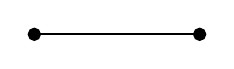
\begin{tikzpicture}[thick, scale=0.7]
    	\tikzstyle{point}=[circle,thick,draw=black,fill=black,inner sep=0pt,minimum width=4pt,minimum height=4pt]
    	\node (a)[point] at (0,0) {};
    	\node (b)[point] at (3,0) {};
 
    	\draw (a.center) -- (b.center) --cycle;
	\end{tikzpicture}
	\caption{1-simplex}\label{ref:1simp}
\end{subfigure}\hspace{0.05\textwidth}
\begin{subfigure}[b]{0.2\textwidth}
\centering
	\begin{tikzpicture}[thick, scale=3]
    	\tikzstyle{point}=[circle,thick,draw=black,fill=black,inner sep=0pt,minimum width=4pt,minimum height=4pt]
    	\coordinate (a) at (0,0);
    	\coordinate (b) at (1,0);
    	\coordinate (c) at (0.6,0.5);

    	\draw[fill=greeo,opacity=0.6] (a) -- (b) -- (c) -- cycle;
 
    	\draw (a) -- (b) -- (c)  --cycle;
    	
    	\node ()[point] at (a) {};
    	\node ()[point] at (b) {};
    	\node ()[point] at (c) {};
	\end{tikzpicture}
	\caption{2-simplex}\label{ref:2simp}
\end{subfigure}\hspace{0.05\textwidth}
\begin{subfigure}[b]{0.2\textwidth}
\centering
	\begin{tikzpicture}[thick,scale=3]
    	\tikzstyle{point}=[circle,thick,draw=black,fill=black,inner sep=0pt,minimum width=4pt,minimum height=4pt]

	\coordinate (A1) at (0,0);
	\coordinate (A3) at (1,0);
	\coordinate (A4) at (0.4,-0.3);
	\coordinate (B1) at (0.5,0.5);

	\draw[thick,dashed,opacity=0.6] (A1) -- (A3);
	\draw[fill=greeo,opacity=0.6] (A1) -- (A4) -- (B1) -- cycle;
	\draw[fill=greeo,opacity=0.6] (A3) -- (A4) -- (B1) -- cycle;

	\draw (A1) -- (B1)  -- (A3) -- (A4) --(A1) --cycle;
	
	\node ()[point] at (A1) {};
	\node ()[point] at (A3) {};
	\node ()[point] at (A4) {};
	\node ()[point] at (B1) {};
	\end{tikzpicture}
	\caption{3-simplex}\label{ref:3simp}
\end{subfigure}
\caption{Representation of 0, 1, 2, and 3-dimensional simplices}
\end{figure}


We can see that any subset of the vertices of $\sigma$ will be affinely independent and will therefore define a lower dimensional simplex $\tau$. Hence, we will say that \emph{$\tau$ is a face of $\sigma$} if it is a convex combination of a non-empty subset of the vertices of $\sigma$, and we will denote it by $\tau \leq \sigma$. If the subset is proper, we will say that \emph{$\tau$ is the proper face of $\sigma$}, and we will denote it by $\tau < \sigma$.\\

Using the definition of faces of a simplex $\sigma$, we can define \emph{the boundary and interior} of $\sigma$.

\begin{definition}
Let a simplex $\sigma$. Then we define
\begin{itemize}
	\item \emph{boundary of $\sigma$} as \[\text{bd } \sigma = \bigcup_{\tau<\sigma}\tau\,.\]
	\item \emph{interior of $\sigma$} as \[\text{int }\sigma= \sigma - \text{bd }\sigma\,.\]
\end{itemize}
\end{definition}

Once we know the pieces of our decomposition, we are going to see how we have to combine them and what are the main properties of the resulting complexes.

As we have already seen at the beginning of the section, for a decomposition to be a complex, its pieces have to be topologically simple, and their intersections have to be lower-dimensional pieces of the same type. The natural way to do this is to glue some simplices together by their faces.

\begin{definition}
A \emph{simplicial complex} is a finite collection of simplices $K$ that satisfy the following properties:
\begin{enumerate}
	\item If $\sigma \in K$ and $\tau \leq \sigma$ then $\tau \in K$.
	\item If $\sigma_0,\sigma_1 \in K$ and $\sigma_0 \cap \sigma_1 \neq \emptyset$ then $\sigma_0 \cap \sigma_1 \leq \sigma_i$ for $i = 1,2$.
\end{enumerate}
\end{definition}

We define the dimension of $K$ as the maximum of its simplices dimensions.

We can see in Figure \ref{ref:comp1} an example of a simplicial complex, while Figure \ref{ref:noComp} shows an example of something that does not verify the abovementioned properties.

\begin{figure}[ht]
\centering
\begin{tikzpicture}[thick,scale=3]
    	\tikzstyle{point}=[circle,thick,draw=black,fill=black,inner sep=0pt,minimum width=4pt,minimum height=4pt]

	\coordinate (x) at (0,0);

	\coordinate (A1) at (1,0);
	\coordinate (A3) at (2, 0.1);
	\coordinate (A4) at (1.4,-0.3);
	\coordinate (B1) at (1.5,0.5);

    \coordinate (b) at (3,0);
    \coordinate (c) at (2.6,-0.5);
    
    \coordinate (a1) at (3.4,0.12);
    \coordinate (b1) at (4,0);
    \coordinate (c1) at (3.8,0.3);
    
    \coordinate (y) at (3.5,-0.4);
	
	\draw[thick,dashed,opacity=0.6] (A1) -- (A3);
    \draw[fill=greeo,opacity=0.6] (a1) -- (b1) -- (c1) -- cycle;
	\draw[fill=greeo,opacity=0.6] (A1) -- (A4) -- (B1) -- cycle;
	\draw[fill=greeo,opacity=0.6] (A3) -- (A4) -- (B1) -- cycle;

	\draw (a1) -- (b1) -- (c1)  --cycle;	
	\draw (A1) -- (B1)  -- (A3) -- (A4) --(A1) --cycle;
	\draw (x) -- (A1) --cycle;	
	\draw (A3) -- (b) -- (c)  --cycle;	
	\draw (b1) -- (y) --cycle;
	\draw (B1) -- (A4) --cycle;
	
	\node ()[point] at (x) {};
	\node ()[point] at (A1) {};
	\node ()[point] at (A3) {};
	\node ()[point] at (A4) {};
	\node ()[point] at (B1) {};
    \node ()[point] at (b) {};
    \node ()[point] at (c) {};
    \node ()[point] at (a1) {};
    \node ()[point] at (b1) {};
    \node ()[point] at (c1) {};
    \node ()[point] at (y) {};	
	
	\end{tikzpicture}
\caption{Example of a simplicial complex}
\label{ref:comp1}
\end{figure}

\begin{figure}[ht]
\centering
\begin{tikzpicture}[thick]
    \tikzstyle{point}=[circle,thick,draw=black,fill=black,inner sep=0pt,minimum width=4pt,minimum height=4pt]
    \coordinate (a) at (0,0);
    \coordinate (b) at (3,0);
    \coordinate (c) at (2,2);

    \begin{scope}[yshift=2cm]
    	\coordinate (d) at (1,1);
    	\coordinate (e) at (0,2);
    	\coordinate (f) at (4,2);
    \end{scope}

	\coordinate (p) at (1.5,0.5);

    \draw[fill=greeo,opacity=0.6] (a) -- (b) -- (c) -- cycle;
    \draw[fill=greeo,opacity=0.6] (d) -- (e) -- (f) -- cycle;
    
 
    \draw (p) -- (d) --cycle;
    \draw (a) -- (b) -- (c)  --cycle;
    \draw (d) -- (e) -- (f) -- cycle;    
    
	\node ()[point] at (a) {};
    \node ()[point] at (b) {};
    \node ()[point] at (c) {};
    \node ()[point] at (d) {};
    \node ()[point] at (e) {};
    \node ()[point] at (f) {};
    \node ()[point] at (p) {};    
\end{tikzpicture}
\caption{Example of simplices that does not verify the simplicial complex conditions}
\label{ref:noComp}
\end{figure}

\begin{definition}
The \emph{underlying space} of a simplicial complex $K$, denoted $\abs{K}$, is the union of the simplices in $K$ with the induced topology of $\mathbb{R}^d$ where the simplex are contained. This underlying space is also called \emph{polyhedron}.
\end{definition}
As can be seen, the underlying space of a simplicial complex is compact since it is a finite union of simplices. The following result characterizes the open and closed sets of the underlying space $\abs{K}$ of a simplicial complex $K$.

\begin{proposition}[{\cite[Chapter~3]{edelsbrunner_computational_2010}}]
Let $K$ be a simplicial complex and $A \subset \abs{K}$ a subset. Then $A$ is an open (closed) set in $K$ if and only if for every $\sigma \in K$, $A \cap \abs{\sigma}$ is an open (closed) set of $\abs{\sigma}$.
\end{proposition}

\begin{definition}
A \emph{triangulation} of a topological space $X$ is a pair $(K, h)$ where $K$ is a simplicial complex and $h: X \to \abs{K}$ is a homeomorphism ($h $ continuous, bijective and $h^{-1}$ continuous).
\end{definition}
We will say that a topological space is \emph{triangulable} if it admits triangulation.\\

It will also be helpful for us to be able to study the simplicial complexes contained in another simplicial complex.
\begin{definition}
A \emph{subcomplex} $L$ of a simplicial complex $K$ is a simplicial complex $L \subseteq K$.
\end{definition}

A type of subcomplex of great interest are the \emph{$j$-skeletons}, defined as follows: \[K^{(j)} = \{\sigma \in K \mid dim\ \sigma\ \leq j \}\,.\]

\subsubsection*{Abstract simplicial complexes}
Once we know the simplicial complexes from the geometric point of view, we will approach them from a combinatorial approach, which will significantly help us code the simplicial complexes.

\begin{definition}
An \emph{abstract simplicial complex $A$} is a finite collection of finite sets such that if $\alpha \in A$ and $\beta \subset \alpha$, then $\beta \in A$.
\end{definition}
In this way, it is fulfilled that
\begin{itemize}
    \item Non-empty sets in $A$ are called \emph{abstract simplices}.
    \item The \emph{dimension} of an abstract simplex $\alpha \in A$ is $\text{dim}\ \alpha = \text{card}(\alpha) - 1$. And the dimension of the complex is the maximum of the dimensions of its simplices.
    \item A \emph{face} of $\alpha \in A$ is any non-empty subset of $\beta \subset \alpha$.
    \item The \emph{set of vertices} of $A$, denoted by $\text{Vert } A$, is the union of all its simplices.
    \item A \emph{subcomplex $B$} of an abstract simplicial complex $A$ is an abstract simplicial complex $B \subset A$.
\end{itemize}

\begin{exmp}
The following set forms an abstract simplicial complex:

\begin{gather*}
A = \{\{0\},\{1\},\{2\},\{3\},\{4\},\{5\},\{6\},\{0,1\},\{1,2\},\{1,3\},\{1,4\},\{2,3\},\\
\{2,4\},\{3,4\},\{4,5\},\{4,6\},\{5,6\},\\
\{1,2,3\},\{1,2,4\},\{1,3,4\},\{2,3,4\},\{1,2,3,4\}\}\,.
\end{gather*}

Where the set of vertices is: $\text{Vert }A = \{0, 1, 2, 3, 4, 5, 6\}$.
\end{exmp}

\begin{definition}
Let $A$ and $B$ be two abstract simplicial complexes. We say that $A$ and $B$ are \emph{isomorphic} if there exists a bijection \[b:\text{Vert }A \to \text{Vert }B\] such that $\alpha \in A$ if and only if $b(\alpha) \in B$.
\end{definition}

Each geometric complex naturally induces an abstract complex in the following way:
\begin{definition}
Let $K$ be a simplicial complex, and let $V$ be the set of vertices of $K$. Then, we will call \emph{vertex scheme} the abstract simplicial complex $A$ formed by all those subsets of $V$ that generate simplices in $K$.
\end{definition}

And under certain circumstances, we can do the opposite step of constructing a (geometric) simplicial complex from an abstract one:
\begin{definition}
Let $A$ be an abstract simplicial complex and $K$ a simplicial complex. We will say that $K$ is a \emph{geometric realization} of $A$ if $A$ is isomorphic to the vertex scheme of $K$.
\end{definition}

\begin{theorem}[{\cite[Chapter~3]{edelsbrunner_computational_2010}}]
Every abstract simplicial complex of dimension $d$ admits a geometric realization in $\mathbb{R}^{2d + 1}$.
\end{theorem}

Thus, abstract simplicial complexes are a faithful representation of (geometric) simplicial complexes.

\subsection{Simplicial complexes build from point clouds}
From the computational point of view, we find ourselves with the problem that we have a representation of a topological space through a finite discretization, and our objective is to be able to recover properties of the original topological space from this cloud of points. Hence, to give some structure to our distance space $(X,d)$, where $X$ is the dataset and $d: X \to \overline{\mathbb{R}}_+$ is a distance function, we will create a simplicial complex with the data points as vertices, and encoding some of the relevant information of $d$.

\subsubsection*{\v{C}ech complex}
The \v{C}ech complex is defined from the intersection of a collection of disks (closed balls). The idea underlying this construction is that of the nerve of a collection, which is introduced below.

\begin{definition}
Let $F$ be a finite collection of sets. The \emph{nerve} of F is defined as the abstract simplicial complex
\[
{\rm Nrv}\ F= \left\{ X \subseteq F \mid \bigcap_{x\in X} x \neq \emptyset \right\}\,.
\]
\end{definition}

One of the reasons we are interested in simplicial complexes constructed through the nerve of a collection is based on the implications of the following theorem.

\begin{theorem}[Nerve theorem {\cite[Chapter~3]{edelsbrunner_computational_2010}}]
If $F$ is a finite collection of closed and convex subsets in Euclidean space, then the rib of $F$ has the same type of homotopy as the union of the sets of $F$.
\end{theorem}
Therefore, by this theorem, we know that \v{C}ech complexes ``behaves similarly'' to subsets of $\mathbb{R}^d$ (since it is homopoty equivalent). This property will ensure us that our analysis of the topological properties obtained through homology groups of our simplicial complex will be the same as if we studied them on neighborhoods of our dataset $X\subset \mathbb{R}^d$ \cite{doherty_cech_2018}. \todo{check this claim}\\

We consider the particular case in which the sets of the family are the disks, i.e. closed balls, $D_r(x)\equiv\overline{B_r}(x)= \{y\in \mathbb{R}^d \mid d(x, y) \leq r\}$ in $\mathbb{R}^d$.

\begin{definition}
Let $X\subset \mathbb{R}^d$ be a finite set of points. We will call \emph{\v{C}ech complex} of $X$ of radius $r$ to the abstract simplicial complex
\[
\text{\v{C}ech}(r)=\left\{\sigma \subset X \mid \bigcap_{u \in \sigma} D_{r/2}(u)\neq \emptyset \right\}\,.
\]
\end{definition}

\begin{figure}[!ht]
\centering
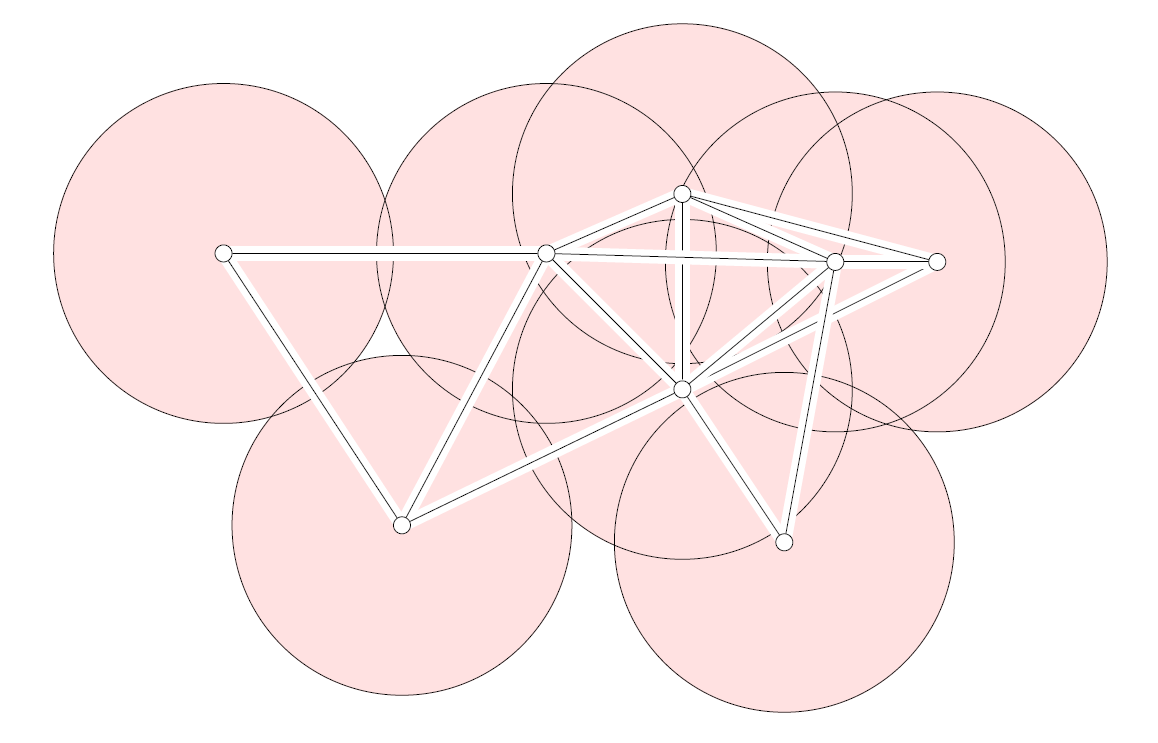
\includegraphics[width=0.5\textwidth]{figures/bg/Cech.png} 
\caption{\v{C}ech complex for a set of nine points and a radius $r$. Source: \cite{edelsbrunner_computational_2010}}
\label{ref:cech}
\end{figure}

We can check that for large enough values of $r$, $\text{\v{C}ech}(r)$ is a simplex of dimension $\text{card }(X)-1$ {\cite[Chapter~3]{edelsbrunner_computational_2010}}, so the \v{C}ech complex is computationally inefficient.

Furthermore, in general, the \v{C}ech complex of a set of points $X \subset \mathbb{R}^d$ does not possess a geometric realization in $\mathbb{R}^d$. Therefore, we will present a construction that resembles the \v{C}ech complex but will be much more favorable from a computational point of view.

\subsubsection*{Vietoris-Rips complex}

\begin{definition}
Let $X \subset \mathbb{R}^d$ be a finite set of points. We call \emph{Vietoris-Rips} complex of $X$ of radius $r$ to the abstract simplicial complex 
\[
\text{VR}(r) = \{\sigma \subseteq  X \mid \textrm{diam } \sigma \leq r\} = \left\{ \{x_0, ..., x_n\} \subseteq  X \mid d(x_i, x_j) \leq r\ \forall i,j\right\}
\]
\end{definition}

We can see in Figure \ref{ref:vr} how the various VR complexes are generated as the radius increases.

\begin{figure}[!ht]
\centering
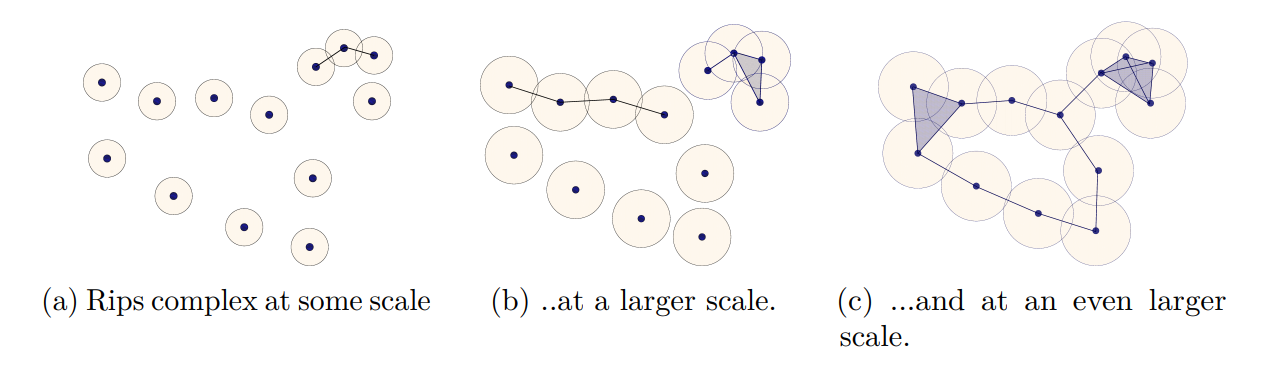
\includegraphics[width=0.9\textwidth]{figures/bg/vr.png} 
\caption{Vietoris-Rips complexes for a set of seven points as we increase the radius from left to right. Source: \cite{ulmer_topological_2019}}
\label{ref:vr}
\end{figure}


Let $\sigma \subset X$, then we remember that the diameter is defined as
\[\textrm{diam } \sigma = \max_{u,v \in \sigma} d(u,v)\,.\]
This observation guarantees that $\sigma \in \text{VR}(r)$ if and only if all its edges are in $\text{VR}(r)$. In other words, $\text{VR}(r)$ is completely determined by its $1$-skeleton. This makes the Vietoris-Rips complex much more efficient than the \v{C}ech complex from the computational point of view. However, as with the \v{C}ech complex, it does not admit a geometric realization in $\mathbb{R}^d$.

On the other hand, the Vietoris-Rips complex is not the nerve of any collection of subsets of $\mathbb{R}^d$. However, the following result guarantees that the VR complex approximates the \v{C}ech complex.

\begin{lemma}[Vietoris-Rips lemma {\cite[Chapter~3]{edelsbrunner_computational_2010}}]
\label{ref:lemaVR}
Let $X \subset \mathbb{R}^d$ be a finite set of points and let $r \geq 0$. Then,
\[
\text{\rm \v{C}ech}(r) \subset \text{\rm VR}(r) \subset \text{\rm \v{C}ech}(\sqrt{2}r)\,.
\]
\end{lemma}


Another important property regarding VR complexes is their ability to encode $\epsilon$-connectivity. We will talk more in detail about $\epsilon$-connectivity and how it will be a crucial property for constructing our topological regularization. 

\begin{definition}[\cite{robins_resolutions_2000}]
We say that a metric space $X$ is \emph{$\epsilon$-disconnected} if there exist two subsets $U$ and $V$ with $U\cup V = X$, and $d(U,V)\equiv \inf_{x\in U, y\in V}d(x,y) \geq \epsilon$.
\end{definition}
Hence if the space is not $\epsilon$-disconnected, we will say that $X$ is $\epsilon$-connected. Moreover, a subset $A \subset X$ is an \emph{$\epsilon$-component} if $A$ is $\epsilon$-connected and $d(A, X \setminus A)\geq \epsilon$. Hence, for any given $\epsilon$, we can decompose our dataset $X$ in disjoint $\epsilon$-components.

However, to see the connection of VR complex with $\epsilon$-connectivity, we will use another definition based on \emph{$\epsilon$-chains}.

\begin{definition}[\cite{robins_resolutions_2000}]
We call \emph{$\epsilon$-chain} to a finite sequence of points $x_0, .., x_n$ such as $d(x_i, x_{i+1})<\epsilon$ for $i=1,...,n$. 
\end{definition}

Therefore, for any set $X$, if we can form an \emph{$\epsilon$-chain} between any pair of points, then our set is $\epsilon$-connected. 

\begin{proposition}
For any distance $d$ on $X$, and $\epsilon \geq 0$, the partition corresponding to the connected components of $VR(\epsilon)$, denoted as $\pi_0(VR(\epsilon))$, coincides with the $\epsilon$-components of $X$.
\end{proposition}

This can be easily seen since two points $u,v$ (vertices) are in the same connected component of a simplicial complex $K$ if there exists a sequence of vertices $u=x_0,..., x_n=v$ such as $\{x_i, x_{i+1}\} \in K$. So, we can see that in the case that $K$ is a Vietoris-Rips complex of radius $\epsilon$, then $\{x_i, x_{i+1}\} \in K$ iff $d(x_i, x_{i+1})<\epsilon$, i.e, there exist an $\epsilon$-chain between $u$ and $v$. \todo{not true since distance for edges should be leq. How do we reflect the inequality? With the limit?}

\subsubsection*{Witness complex}






\subsection{Homology}
As can be seen in \cite{hatcher_algebraic_2002}, the homotopy is an algebraic tool to obtain properties of topological spaces. However, the methods for calculating the homotopy are not computationally manageable. Thus, homology is proposed as an algebraic formalism, which, although it is not capable of obtaining as much topological information about space as with other formalisms, it is highly beneficial from a computational perspective.

We will start by reviewing some linear algebra concepts that will be useful to fully understand the homology's formal definition.

\subsubsection*{Linear algebra interlude}
This subsection is based on Wojciech Chachólski's lecture notes of his course on Topological Data Analysis \cite{chacholski_sf2956_2022}.\\

In TDA we tend to use vector spaces over $F_2$, the field with 2 elements $\{0,1\}$. This field is isomorphic to $\mathbb{Z}_2 \equiv \mathbb{Z}/2\mathbb{Z}$ with operations modulo 2:
\[
0+0 = 0;\ 1+0 = 1;\ 1+1 = 0;\ 1 \cdot 0 = 0;\ 1\cdot 1 = 1\,.
\]

We recall that an $F_2$ vector space is a set $V$ with a zero element $0 \in V$ and an addition operation $V \times V \ni (v,w) \mapsto v+w \in V$ such that, for any $u,v,w$ in $V$:
\begin{itemize}
    \item $v + w = w + v$,
    \item $(v + u) + w = v + (u + w)$,
    \item $0 + v = v$,
    \item $v + v = 0$.
\end{itemize}

Another vector spaces that we will use are \emph{quotient spaces}. Let $W \subset V$ be a vector subspace. We define the following equivalence relation: we say that two elements $v$ and $w$ in $V$ are \emph{equivalent modulo} $W$ if $v-w \in W$. As we can see in Figure \ref{fig:quot_ex} the equivalence classes are of the form $[v]=v+W \subset V$. Moreover, the set of equivalence classes, denoted by $V/W$, with the following operations is a vector space:
\begin{itemize}
    \item $(v+W)+(w+W)=v+w+W$,
    \item $0 = 0 +W = W$,
    \item $a(v+W)=av +W$.
\end{itemize}

\begin{figure}[ht!]
    \centering
    \begin{tikzpicture}[line cap=round,line join=round,>=triangle 45,x=1cm,y=1cm]
        \begin{axis}[
        x=1cm,y=1cm,
        axis lines=middle,
        ymajorgrids=true,
        xmajorgrids=true,
        xmin=-3.5771885955480864,
        xmax=4.11169202904735,
        ymin=-2.6112285059644633,
        ymax=3.610515886376021,]
        \clip(-3.5771885955480864,-2.6112285059644633) rectangle (4.11169202904735,3.610515886376021);
        \draw [line width=2pt,color=qqqqff,domain=-3.5771885955480864:4.11169202904735] plot(\x,{(--8.32--4*\x)/4});
        \draw [line width=2pt,color=wwzzqq,domain=-3.5771885955480864:4.11169202904735] plot(\x,{(--15.76--4*\x)/4});
        \draw [line width=2pt,color=ffqqqq,domain=-3.5771885955480864:4.11169202904735] plot(\x,{(-8.4--4*\x)/4});
        \draw [->,line width=1pt,color=qqqqff] (0,0) -- (-1.04,1.04);
        \draw [->,line width=1pt,color=wwzzqq] (0,0) -- (-0.6041708999218006,3.3358291000781994);
        \draw [->,line width=1pt,color=ffqqqq] (0,0) -- (2.1,0);
        \draw [line width=2pt,domain=-3.5771885955480864:4.11169202904735] plot(\x,{(-0--4*\x)/4});
        \begin{scriptsize}
        \draw[color=black] (-2.2934443923249974,-1.9829409990960194) node {$W$};
        \draw[color=qqqqff] (-2.7,-1.2) node {$[u]$};
        \draw[color=wwzzqq] (-2.7,0.6) node {$[v]$};
        \draw[color=ffqqqq] (0.5,-2.125579243898585) node {$[w]$};
        \draw[color=qqqqff] (-0.6,0.4) node {$u$};
        \draw[color=wwzzqq] (-0.6,2.248660263380096) node {$v$};
        \draw[color=ffqqqq] (1.075535103964169,0.15) node {$w$};
        \end{scriptsize}
        \end{axis}
    \end{tikzpicture}
    \caption{Quotient space example: $\mathbb{R}^2/W$}
    \label{fig:quot_ex}
\end{figure}

Lastly, we will see that one of our main components for constructing homology is by ``transforming'' a set to a vector space. Hence, for any finite set $X$, and field $F$, we define $FX \equiv \oplus_{x \in X} K$. The vector space $FX$ is isomorphic to $F^{\abs{X}}$, which means that we can represent an element of $FX$ as sequences $(k_x)_{x \in X}$ indexed by elements of X.

\begin{exmp}
Let the set $S=\{a, b, c\}$, and the field $F_4$. Then an element of $F_4S$ can be
\[
( \underbrace{1}_\text{a}, \underbrace{0}_\text{b}, \underbrace{2}_\text{c}) = 1 \cdot a + 0 \cdot b + 2 \cdot c = a + 2c\,.
\]
\end{exmp}

Therefore, we can see that we can define a basis for this space formed by elements $e_x$, where

\[
(e_x)_y = \left\{\begin{matrix}
1 & \text{ if } y=x\\
1 & \text{ if } y \neq x\\
\end{matrix}\right.
\]

So the notation that we have seen in the example of representing an element as a (unique) linear combination $\sum_{x \in X} a_x x$ can be formalized if we identify each element $x$ in $X$ with $e_x$. Furthermore, given two elements $c = \sum_{x \in X} a_x x$ and $c' = \sum_{x \in X} b_x x$, their sum is defined as
\[
c + c' = \sum_{x \in X} (a_x + b_x) x\,.
\]

Lastly, we will see that we can extend a map of sets $g:X \to Y$ to a linear equation $Fg: KX \to KY$ such as an element $\sum_{x \in X} a_x x$ will be mapped to $\sum_{x \in X} a_x g(x)$.


\subsubsection*{Chain groups}
We will begin by studying the various groups that are involved in the definition of homology.


Let $K$ be a simplicial complex, $F$ a field, and $p$ be a non-negative integer. A \emph{$p$-chain} in $K$ is equal to $FK$. More specifically, $c$ is a $p$-chain in $K$ if
\[
c = \sum a_i\sigma_i
\]
with $\sigma_i$ is a $p$-simplex for each $i$ and $a_i$ are the \emph{coefficients}. These coefficients can be taken from any commutative ring $F$; however, we will use coefficients in the field of two elements, i.e.,  $a_i \in \mathbb{Z}_2$.

\begin{exmp}
We will write the simplices as the list of their vertices, $\sigma = [u_0, u_1, ..., u_p]$.
\begin{itemize}
	\item In the figure \ref{ref:0cad} the $0$-chain $c=[0]+[2]+[6]+[9]$ is shown in red.
\begin{figure}[!ht]
\centering
\begin{tikzpicture}[thick,scale=3]
    	\tikzstyle{point}=[circle,thick,draw=black,fill=black,inner sep=0pt,minimum width=4pt,minimum height=4pt]
    	\tikzstyle{point1}=[circle,thick,draw=black,fill=red,inner sep=0pt,minimum width=7pt,minimum height=7pt]

	\coordinate (x) at (0,0);

	\coordinate (A1) at (1,0);
	\coordinate (A3) at (2, 0.1);
	\coordinate (A4) at (1.4,-0.3);
	\coordinate (B1) at (1.5,0.5);

    \coordinate (b) at (3,0);
    \coordinate (c) at (2.6,-0.5);
    
    \coordinate (a1) at (3.4,0.12);
    \coordinate (b1) at (4,0);
    \coordinate (c1) at (3.6,0.3);
    
    \coordinate (y) at (3.5,-0.4);
	
	\draw[thick,dashed,opacity=0.6] (A1) -- (A3);
    \draw[fill=greeo,opacity=0.6] (b) -- (b1) -- (c1) -- cycle;
	\draw[fill=greeo,opacity=0.6] (A1) -- (A4) -- (B1) -- cycle;
	\draw[fill=greeo,opacity=0.6] (A3) -- (A4) -- (B1) -- cycle;

	\draw (b) -- (b1) -- (c1)  --cycle;	
	\draw (A1) -- (B1)  -- (A3) -- (A4) --(A1) --cycle;
	\draw (x) -- (A1) --cycle;	
	\draw (A3) -- (b) -- (c)  --cycle;	
	\draw (b1) -- (y) --cycle;
	\draw (B1) -- (A4) --cycle;	
	
	\node ()[point1,label={$0$}] at (x) {};
	\node ()[point,label={$1$}] at (A1) {};
	\node ()[point1,label={$2$}] at (B1) {};
	\node ()[point,label={[shift={(0.3,-0.5)}]$3$}] at (A4) {};
	\node ()[point,label={$4$}] at (A3) {};
	\node ()[point,label={$5$}] at (c) {};
    \node ()[point1,label={$6$}] at (b) {};
    \node ()[point,label={$7$}] at (c1) {};
    \node ()[point,label={$8$}] at (b1) {};
    \node ()[point1,label={$9$}] at (y) {};	
	
	\end{tikzpicture}
\caption{Example of $0$-chain}
\label{ref:0cad}
\end{figure}
	\item In the figure \ref{ref:1cad} the $1$-chain $c=[0,1]+[1,2]+[2,4]+[8,9]$ is shown in red.
\begin{figure}[!ht]
\centering
\begin{tikzpicture}[thick,scale=3]
    	\tikzstyle{point}=[circle,thick,draw=black,fill=black,inner sep=0pt,minimum width=4pt,minimum height=4pt]
    	\tikzstyle{point1}=[circle,thick,draw=black,fill=red,inner sep=0pt,minimum width=7pt,minimum height=7pt]
    	\tikzstyle{line}=[line width=1.5pt, red]

	\coordinate (x) at (0,0);

	\coordinate (A1) at (1,0);
	\coordinate (A3) at (2, 0.1);
	\coordinate (A4) at (1.4,-0.3);
	\coordinate (B1) at (1.5,0.5);

    \coordinate (b) at (3,0);
    \coordinate (c) at (2.6,-0.5);
    
    \coordinate (a1) at (3.4,0.12);
    \coordinate (b1) at (4,0);
    \coordinate (c1) at (3.6,0.3);
    
    \coordinate (y) at (3.5,-0.4);
	
	\draw[thick,dashed,opacity=0.6] (A1) -- (A3);
    \draw[fill=greeo,opacity=0.6] (b) -- (b1) -- (c1) -- cycle;
	\draw[fill=greeo,opacity=0.6] (A1) -- (A4) -- (B1) -- cycle;
	\draw[fill=greeo,opacity=0.6] (A3) -- (A4) -- (B1) -- cycle;

	\draw (b) -- (b1) -- (c1)  --cycle;	
	\draw (A1) -- (B1)  -- (A3) -- (A4) --(A1) --cycle;
	\draw (A3) -- (b) -- (c)  --cycle;	
	\draw[line] (b1) -- (y) --cycle;
	\draw[line] (x) -- (A1) -- (B1) -- (A3);	
	\draw (B1) -- (A4) --cycle;
	
	\node ()[point1,label={$0$}] at (x) {};
	\node ()[point1,label={$1$}] at (A1) {};
	\node ()[point1,label={$2$}] at (B1) {};
	\node ()[point,label={[shift={(0.3,-0.5)}]$3$}] at (A4) {};
	\node ()[point1,label={$4$}] at (A3) {};
	\node ()[point,label={$5$}] at (c) {};
    \node ()[point,label={$6$}] at (b) {};
    \node ()[point,label={$7$}] at (c1) {};
    \node ()[point1,label={$8$}] at (b1) {};
    \node ()[point1,label={$9$}] at (y) {};	
	
	\end{tikzpicture}
\caption{Example of $1$-chain}
\label{ref:1cad}
\end{figure}
	\item In the figure \ref{ref:2cad} the $2$-chain $c=[1,2,3] + [2,3,4] + [6,7,8]$ is shown in red.
\begin{figure}[!ht]
\centering
\begin{tikzpicture}[thick,scale=3]
    	\tikzstyle{point}=[circle,thick,draw=black,fill=black,inner sep=0pt,minimum width=4pt,minimum height=4pt]
    	\tikzstyle{point1}=[circle,thick,draw=black,fill=red,inner sep=0pt,minimum width=7pt,minimum height=7pt]
    	\tikzstyle{line}=[line width=1.5pt, red]
    	
	\coordinate (x) at (0,0);

	\coordinate (A1) at (1,0);
	\coordinate (A3) at (2, 0.1);
	\coordinate (A4) at (1.4,-0.3);
	\coordinate (B1) at (1.5,0.5);

    \coordinate (b) at (3,0);
    \coordinate (c) at (2.6,-0.5);
    
    \coordinate (a1) at (3.4,0.12);
    \coordinate (b1) at (4,0);
    \coordinate (c1) at (3.6,0.3);
    
    \coordinate (y) at (3.5,-0.4);
	
	\draw[thick,dashed,opacity=0.6,line] (A1) -- (A3);
    \draw[fill=redp,opacity=0.6] (b) -- (b1) -- (c1) -- cycle;
	\draw[fill=redp,opacity=0.6] (A1) -- (A4) -- (B1) -- cycle;
	\draw[fill=redp,opacity=0.6] (A3) -- (A4) -- (B1) -- cycle;

	\draw[line] (b) -- (b1) -- (c1)  --cycle;	
	\draw[line] (A1) -- (B1)  -- (A3) -- (A4) --(A1) --cycle;
	\draw (x) -- (A1) --cycle;	
	\draw (A3) -- (b) -- (c)  --cycle;	
	\draw (b1) -- (y) --cycle;
	\draw[line] (B1) -- (A4) --cycle;

	
	\node ()[point,label={$0$}] at (x) {};
	\node ()[point1,label={$1$}] at (A1) {};
	\node ()[point1,label={$2$}] at (B1) {};
	\node ()[point1,label={[shift={(0.3,-0.5)}]$3$}] at (A4) {};
	\node ()[point1,label={$4$}] at (A3) {};
	\node ()[point,label={$5$}] at (c) {};
    \node ()[point1,label={$6$}] at (b) {};
    \node ()[point1,label={$7$}] at (c1) {};
    \node ()[point1,label={$8$}] at (b1) {};
    \node ()[point,label={$9$}] at (y) {};	
	
	\end{tikzpicture}
\caption{Example of $2$-chain}
\label{ref:2cad}
\end{figure}
\end{itemize}
\end{exmp}


The $p$-chains with the operation addition $+$ form the \emph{group of $p$-chains} denoted by $(\text{C}_p,+)$, but since the operation is understood, it is usually represented as $\text{C}_p=\text{C}_p(K)$.

This group is an abelian group, and as we have seen above, $\text{C}_p(K)$ is a vector space over $\mathbb{Z}_2$. Hence, fixed $p \in \mathbb{Z}$, a basis of the vector space $\text{C}_p(K)$ is the set $\{\sigma_i^p \mid i=1,...,s_p\}$ formed by the simplices of dimension $p$ of $K$. As a consequence $\text{C}_p(K)=\{0\}$, where $0 = \sum 0\cdot\sigma_i$, if $p < 0$ or $p > \text{dim}(K)$.

\subsubsection*{Boundary operator}
To be able to relate these groups, we will define the \emph{boundary operator}. Therefore, we will start with the definition of the $p$-boundary of a simplex.

\begin{definition}
Let $p$ be an integer and $\sigma \in K$ be a $p$-simplex $\sigma = [v_0, v_1, ..., v_p]$ its \emph{$p$-boundary} is defined, $\partial_p\sigma$, as the formal sum its $(p-1)$-dimensional faces, that is,
\[
\partial_p\sigma = \sum_{j=0}^{p}[v_0, ..., \hat{v}_j, ..., v_p]
\]
where $\hat{v}_j$ denotes that $v_j$ is omitted.
\end{definition}

In general, given a $p$-chain $c =\sum a_i\sigma_i$, its $p$-boundary is defined by linear extension as $\partial_p c= \sum_{j=0}^{p} a_i \partial_p \sigma_i $. As a consequence, the boundary defines a linear mapping $\partial_p: \text{C}_p \to \text{C}_{p-1}$ between vector spaces of chains called the \emph{boundary operator}. To simplify the notation, the subscript $p$ of the boundary operator is often omitted since it always matches the dimension of the chain to which it is applied.


\begin{exmp}
Let $c = [0,1] + [4,5]$ a $2$-chain, then the boundary of $c$ is:
\[
\partial c = \partial [0,1] + \partial [4,5] = [0] + [1] + [4] + [5]\,.
\]
\end{exmp}

\subsubsection*{Cycles and boundaries}
We will distinguish two types of chains, which we will use to define homology groups.
\begin{definition}
We say that a $p$-chain $c$ is a \emph{$p$-cycle} if
\[
\partial c = 0
\]
or, equivalently, if $c \in \text{ker }\partial$.
\end{definition}

Because $\partial$ commutes with addition $+$, 

\begin{exmp}
We will see that geometrically, the $p$-cycles represent cycles in the simplicial complex. These, in turn, can be holes of dimension $p$. In the figure \ref{ref:1-ciclo} the $1$-cycle $[4,5] + [4,6] + [5,6]$ is shown in red, which is a hole. While blue represents the $1$-cycle $[6,7] + [6,8] + [7,8]$, which is not a hole.

\begin{figure}[!ht]
\centering
\begin{tikzpicture}[thick,scale=3]
    	\tikzstyle{point}=[circle,thick,draw=black,fill=black,inner sep=0pt,minimum width=4pt,minimum height=4pt]
    	\tikzstyle{point1}=[circle,thick,draw=black,fill=red,inner sep=0pt,minimum width=7pt,minimum height=7pt]
    	\tikzstyle{point2}=[circle,thick,draw=black,fill=blue,inner sep=0pt,minimum width=7pt,minimum height=7pt]
    	\tikzstyle{line}=[line width=1.5pt, red]
    	\tikzstyle{line1}=[line width=1.5pt, blue]

	\coordinate (x) at (0,0);

	\coordinate (A1) at (1,0);
	\coordinate (A3) at (2, 0.1);
	\coordinate (A4) at (1.4,-0.3);
	\coordinate (B1) at (1.5,0.5);

    \coordinate (b) at (3,0);
    \coordinate (c) at (2.6,-0.5);
    
    \coordinate (a1) at (3.4,0.12);
    \coordinate (b1) at (4,0);
    \coordinate (c1) at (3.6,0.3);
    
    \coordinate (y) at (3.5,-0.4);
	
	\draw[thick,dashed,opacity=0.6] (A1) -- (A3);
    \draw[fill=greeo,opacity=0.6] (b) -- (b1) -- (c1) -- cycle;
	\draw[fill=greeo,opacity=0.6] (A1) -- (A4) -- (B1) -- cycle;
	\draw[fill=greeo,opacity=0.6] (A3) -- (A4) -- (B1) -- cycle;

	\draw (b) -- (b1) -- (c1)  --cycle;	
	\draw (B1) -- (A3) -- (A4);
	\draw[line1] (A1) -- (B1) -- (A4) --cycle;
	\draw[line] (A3) -- (b) -- (c)  --cycle;	
	\draw (b1) -- (y) --cycle;
	\draw (x) -- (A1);	

	
	\node ()[point,label={$0$}] at (x) {};
	\node ()[point2,label={$1$}] at (A1) {};
	\node ()[point2,label={$2$}] at (B1) {};
	\node ()[point2,label={[shift={(0.3,-0.5)}]$3$}] at (A4) {};
	\node ()[point1,label={$4$}] at (A3) {};
	\node ()[point1,label={$5$}] at (c) {};
    \node ()[point1,label={$6$}] at (b) {};
    \node ()[point,label={$7$}] at (c1) {};
    \node ()[point,label={$8$}] at (b1) {};
    \node ()[point,label={$9$}] at (y) {};	
	
	\end{tikzpicture}
\caption{Example of $1$-cycle}
\label{ref:1-ciclo}
\end{figure}
\end{exmp}


\begin{definition}
\begin{sloppypar}
We say that a $p$-chain $c$ is an \emph{$p$-boundary} if there exists a $(p+1)$-chain $c'$ such that
\[
\partial c' = c
\]
or, equivalently, if $c \in \text{im }\partial_{p+1}$.
\end{sloppypar}
\end{definition}

\begin{exmp}
The $1$-cycle that we had highlighted in blue in the Figure \ref{ref:1-ciclo} is a $1$-boundary.
\end{exmp}

\begin{remark}
The sets of $p$-cycles $\text{Z}_p = \text{ker }\partial_p$, and $p$-boundaries $\text{B}_p = \text{im }\partial_{p+1} $ are linear subspaces of $\text{C}_p$.
\end{remark}

We will prove that the $p$-boundaries are $p$-cycles, as in the previous example. For this, we will state the following lemma.

\begin{lemma}[Fundamental lemma of homology {\cite[Chapter~4]{edelsbrunner_computational_2010}}]
$\partial_p \partial_{p+1} c = 0$ for every integer $p$ and every $(p + 1)$-chain $c$.
\end{lemma}

It follows that $\text{B}_p$ is a vector subspace of $\text{Z}_p$, that is, $\text{B}_p \subset \text{Z}_p$. Furthermore, we can define the \emph{chain complex} associated with a simplicial complex $K$ as the succession of chain groups connected by the boundary operators
\[
...\overset{\partial_{p+2}}{\longrightarrow}\text{C}_{p+1}\overset{\partial_{p+1}}{\longrightarrow}\text{C}_ {p}\overset{\partial_{p}}{\longrightarrow}\text{C}_{p-1}\overset{\partial_{p-1}}{\longrightarrow}...
\]

We can see in Figure \ref{ref:gruposCadenasOpBorde} this relationship between the chain group $\text{C}_p$, the group of cycles $\text{Z}_p$ and the group of boundaries $\text{B}_p $; and its connections generated by the boundary operator.

\begin{figure}[!ht]
\centering
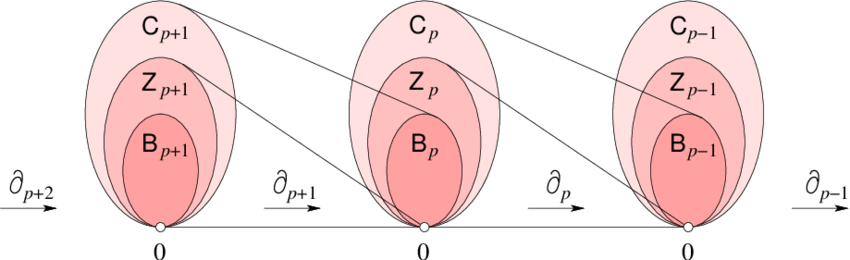
\includegraphics[width=0.8\textwidth]{figures/bg/chain_complex.png} 
\caption{Chain complex representing the chain group, the cycle group, and the boundary group. Source: \cite{edelsbrunner_computational_2010}}
\label{ref:gruposCadenasOpBorde}
\end{figure}


\subsubsection*{Simplicial homology}
The main idea of simplicial homology groups is to be able to find the holes by making use of the cycles. To do this, we will have to ``discard'' those cycles that are boundaries. This is why we will quotient the group of cycles by the group of boundaries since then, all the boundaries will be trivial in homology.

\begin{definition}
Given a simplicial complex $K$, its \emph{$p$-dimensional simplicial homology group} is defined as the quotient space
\[
\text{H}_p(K)=\dfrac{\text{Z}_p}{\text{B}_p}\,.
\]
The \emph{$p$-dimensional Betti number $\beta_p(K)$} is defined as the dimension of $\text{H}_p(K)$.
\end{definition}

Hence, the elements $z \in \text{H}_p = \text{H}_p(K)$ are of the form $z = c + \text{B}_p$ with $c \in \text{Z}_p$, where $c + \text{B}_p$ is the \emph{coset} of $\text{B}_p$ in $\text{Z}_p$. Two cycles $c_1, c_2 \in \text{Z}_p$ represent the same \emph{homology class} $z \in \text{H}_p$ if and only if $z= c_1 + \text{B} _p = c_2 + \text{B}_p$; which is equivalent to $(c_1-c_2) \in \text{B}_p$.

\begin{definition}
We say that two cycles $c_1, c_2 \in \text{Z}_p$ are \emph{homologous} if there exists $b \in \text{B}_p$ such that
\[
c_1 = c_2 + b\,.
\]
\end{definition}

Also, since $\text{Z}_p$, $\text{B}_p$, and $\text{H}_p$ are vector spaces over $\mathbb{Z}_2$ it follows that
\[
\beta_p = \text{dim } \text{H}_p = \text{dim } \text{Z}_p - \text{dim } \text{B}_p\,.
\]


\subsubsection*{Topological properties}

One of the most important values regarding homology groups is their corresponding Betti numbers, as these will give us a lot of information about the underlying space.
\begin{theorem}[{\cite[Proposition~2.7]{hatcher_algebraic_2002}}]
Let $K$ be a simplicial complex. Then $\beta_0(K)$ matches the number of connected components of $\abs{K}$.
\end{theorem}

\begin{corollary}
$\abs{K}$ is connected if and only if $\beta_0(K)=1$.
\end{corollary}

We will see that our topological regularization will exploit the ability to study connectivity through homology. However, we can extract higher dimensional topological properties if we use higher dimensional homology groups. The \emph{Alexander duality theorem} \cite[Chapter~5]{edelsbrunner_computational_2010} allows us to interpret the Betti numbers of a polyhedron contained in $\mathbb{R}^3$: \todo{not sure if is this theorem}
\begin{itemize}
\item $\beta_0(K)$ tells us the number of connected components.
\item $\beta_1(K)$ tells us the number of tunnels.
\item $\beta_2(K)$ indicates the number of cavities.
\end{itemize}

In conclusion, the $p$-homology groups will represent $p$-dimensional holes in topological spaces.

\subsection{Persistence}
We will introduce the concept of persistence first for functions of one variable and then we will deepen in the case of simplicial complexes. In this section, I will use \cite{goodman_persistent_2008} as our main reference.

\subsubsection*{One-dimensional real functions}
Let $f: \mathbb{R} \to \mathbb{R}$ be a smooth function. Remember that $x$ is a \emph{critical point} and $f(x)$ is a \emph{critical value of $f$} if $f'(x)=0$. Furthermore, a critical point $x$ is \emph{non-degenerate} if $f''(x) \neq 0$. So, suppose that $f$ contains only non-degenerate critical points with distinct critical values.\\

Let the \emph{sublevel set} $\mathbb{R}_t=f^{-1}(-\infty, t]$ for each $t \in \mathbb{R}$. Then we see that as we increase $t$, the number of connected components of $\mathbb{R}_t$ will remain constant until we pass through a $t_0$ critical value of $f$.  As we can see in the figure \ref{ref:sublevelR}, when we pass through a local minimum, a new connected component is created. When we pass through a local maximum, two connected components are combined into one.\\

\begin{figure}[!ht]
    \centering
    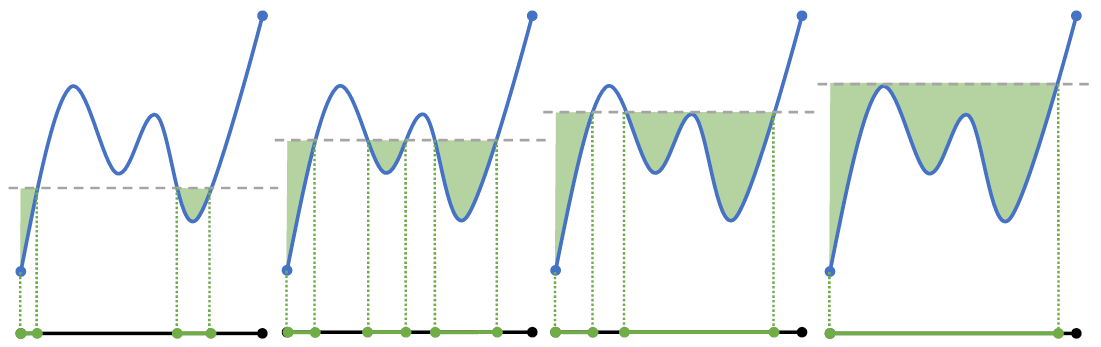
\includegraphics[width=\textwidth]{figures/bg/Sub-level-Filtrations.png}
    \caption{Connected components in $\mathbb{R}$ in the different leaks. Source: \cite{curry_counting_2020}}
    \label{ref:sublevelR}
\end{figure}

The critical points of $f$ are paired as follows:
\begin{enumerate}
    \item When a new connected component appears, we say that the local minimum that created it \emph{represents} that component.
    \item When we pass through a local maximum and two components meet, we pair the maximum with the higher (youngest) of the two local minima that these components represent. The other minimum (the oldest) becomes the representative of the new component resulting from joining the two previous ones.
\end{enumerate}

When the points $x_1$ and $x_2$ are paired following this method, we define the \emph{persistence} of the pair as $f(x_2) - f(x_1)$. This persistence is coded through the \emph{persistence diagram}, representing each pair with the point $(f(x_1),f(x_2))$, as can be seen in the figure \ref{ref:persistenceR}. It can be seen that all points will lie above the diagonal $y=x$ and that persistence is the vertical distance from a point to the diagonal. For reasons that will be explained later, the points on the diagonal will be added to the persistence diagram.

\begin{figure}[!ht]
\centering
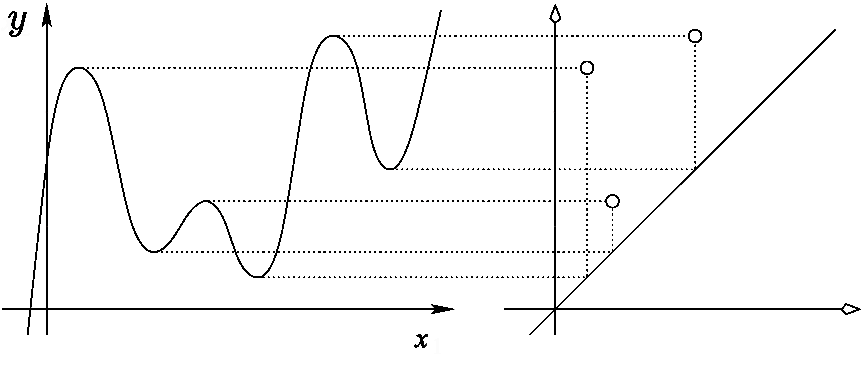
\includegraphics[width=0.8\textwidth]{figures/bg/diagramaR.png} 
\caption{Pairing of the critical points of the function on the left represented as points in the persistence diagram on the right. Modified from: \cite{goodman_persistent_2008}}
\label{ref:persistenceR}
\end{figure}


\subsubsection*{Persistence on simplicial complexes}
We will see that we can expand the concept of persistence seen for real functions to simplicial complexes. To do this, we will use the \emph{filtrations} of a simplicial complex as sub-level sets and we will use the \emph{simplicial homology} as a homology theory.

\begin{definition}
Let $K$ be a simplicial complex and $f: K \to \mathbb{R}$ a function. It is said that, $f$ is \emph{monotonous} if $f(\sigma) \leq f(\tau) $ when $\sigma$ is a face of $\tau$.
\end{definition}
\begin{sloppypar}
The monotony of $f$ guarantees that for every $a \in \mathbb {R}$, the sub-level set ${K(a) = f^{-1} (-\infty, a]} $ is a subcomplex of $K$. As an example, we can define a Vietoris Rips restricted to its 1-skeleton using a monotone function as follows.
\end{sloppypar}

\begin{proposition}[\cite{hofer_connectivity-optimized_2019}]
Let $X$ be a subset of $\mathbb{R}^n$, $\abs{X}=b$, and $\mathcal{V}(X) = \{\sigma \in \mathcal{P}([b]) \mid 1 \leq \abs{\sigma} \leq 2\}$, and define
\[
f_X: \mathcal{V}(X) \to \mathbb{R},\ f_X(\sigma) = \left\{\begin{matrix}
0 &  \text{ if } \sigma=\{i\}\\
\frac{1}{2}d(x_i, x_j) & \text{ if } \sigma=\{i,j\}\\
\end{matrix}\right. 
\]

Then the Vietoris Rips complex w.r.t $r\geq 0 $, restricted to its 1-skeleton is equal to $K_r=f_X^{-1}(-\infty, r]$.
\end{proposition}


\begin{definition}
Let $a_1 <a_2 <... <a_n$ the values that the function takes on the simplices and let $ a_0 = -\infty$. Then $f$ induces a \emph{filtration}
\[
\emptyset = K_0 \xhookrightarrow{} K_1 \xhookrightarrow{} ... \xhookrightarrow{} K_n = K, \text{with } K_i = K (a_i) \,.
\]
\end{definition}
 
Since $K_i \subseteq K_j$ for all indices $i,j$ with $i \leq j$, then the inclusions induce a linear function $f^{i,j}_p: \text{H}_p(K_i) \to \text{H}_p(K_j)$ for all $p$. We could say that this function sees on which homology class of $K_j$ a cycle on $K_i$ will belong. Hence we can formalize the idea of simplicial persistence, making use of these functions.

\begin{definition}
Let ${f_{p}^{i,j}: \text{H}_p(K_i) \to \text{H}_p(K_j)}$ be the linear mapping induced by the inclusion $K_i \subseteq K_j$ . The \emph{persistent homology groups} are defined as the image of $\text{H}_p(K_i)$ in $\text{H}_p(K_j)$ of the map $f_{p}^{i,j}$, that is ,
\[
\text{H}_{p}^{i,j} = \text{im } f_{p}^{i,j}\,.
\]
The corresponding \emph{persistent Betti numbers} are defined as the dimension of these vector spaces,i.e., $\beta_{p}^{i,j} = \text{dim } \text{H}_{p}^{i,j}$.
\end{definition}

\begin{remark}
If we analyze the maps $f_{p}^{i,j}$, we observe that the $\text{ker } f_{p}^{i,j}$ are those elements $\gamma \in \text{H} _p(K_i)$ such that $f_{p}^{i,j}(\gamma)=0$. This means that if $c$ is a cycle representing $\gamma$, then $c \in \text{B}_p(K_j)$. Hence,
\[
\text{ker } f_{p}^{i,j} = \frac{\text{Z}_p(K_i) \cap \text{B}_p(K_j)}{\text{B}_p(K_i)}
\]
for each dimension $p$ fixed. Therefore,

\[
\text{H}_p^{i,j} = \text{im }f_p^{i,j} \cong \frac{\text{H}_p(K_i)}{\text{ker } f_p^{i,j}} = \frac{\frac{\text{Z}_p(K_i)}{\text{B}_p(K_i)}}{\frac{\text{Z}_p(K_i) \cap \text{B}_p(K_j)}{\text{B}_p(K_i)}} \cong \frac{\text{Z}_p(K_i)}{\text{Z}_p(K_i) \cap \text{B}_p(K_j)}\,,
\]
which means that the persistent homology group consists of the classes that were born before $a_i$ and are still alive in $a_j$.
\end{remark}

Comparing this case with the previously shown one in which we used a real function, the critical values of homology are the levels at which the homology of the sublevel sets changes. In this way, we will say that a homology class $\gamma$ is born in $K_i$ if it is not in the image of the function induced by the inclusion $K_{i-1} \subseteq K_i$. Also, a class $\gamma$ that is born in $K_i$ dies when entering $K_j$ if the image of the function induced by $K_{i-1} \subseteq K_{j-1}$ does not contain the image of $\gamma$, but the image of the function induced by $K_{i-1} \subseteq K_j$ does. Which can be formally redefined as follows using persistent homology groups:

\begin{itemize}
\item A class $\gamma \in \text{H}_p(K_i)$ \emph{is born} in $K_i$ if $\gamma \notin \text{H}_p^{i-1, i}$.
\item A class $\gamma \in \text{H}_p(K_i)$ born in $K_i$ \emph{dies} on entering $K_j$ if $f_{p}^{i,j-1}( \gamma)\notin \text{H}_p^{i-1, j-1}$, but $f_p^{i,j}(\gamma)\in \text{H}_p^{i-1, j}$.
\end{itemize}

\begin{definition}
Let $\gamma$ be a homology class that is born in $K_i$ and dies when it enters $K_j$. The \emph{persistence} of $\gamma$ is defined as $\text{pers}(\gamma)= a_j - a_i$. Likewise, the difference $j-i$ is called the \emph{persistence index} of the class $\gamma$. If a class $\gamma$ is born in $K_i$ but never dies, then we say that its persistence, like its index, is infinite.
\end{definition}

Following this notation, the multiplicity is defined as
\[
\mu_p^{i,j} = (\beta_p^{i,j-1}-\beta_p^{i,j})-(\beta_p^{i-1, j-1}-\beta_p^{i-1, j})\,.
\]
Where $\beta_p^{i, j-1}$ can be interpreted as the number of homology classes that are alive in $K_i$ and still alive in $K_{j-1}$. Therefore, the first difference of the equality is interpreted as the number of independent classes that are alive at $K_i$ and die at $K_j$, while the second difference is the number of independent classes that are born before $K_i$ and die in $K_j$. In conclusion, the multiplicity, $\mu_p^{i, j}$, is interpreted as the number of homology classes that are born in $K_i$ and die in $K_j$.


\begin{definition}
The \emph{persistence diagram} $\text{Dgm}(f) \subset \overline{\mathbb{R}}^2$ of $f$ is the multiset of points $(a_i, a_j)$ with multiplicity $ \mu_p^{i, j}$ for all $0 \leq i < j \leq n$, union of diagonal points, $\Delta=\{(x, y) \in \overline{\mathbb{R }}^2 \mid y = x\}$, with infinite multiplicity.
\end{definition}

\begin{figure}[!ht]
\centering
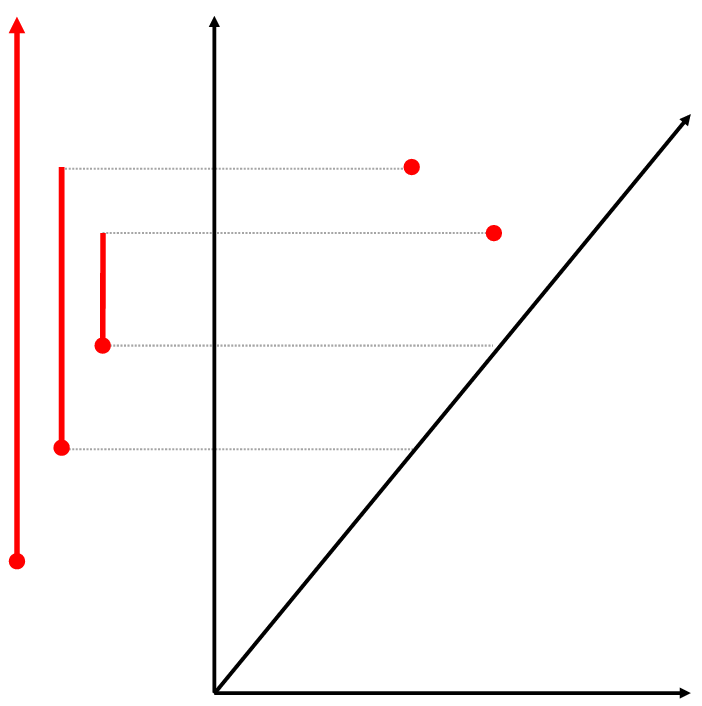
\includegraphics[width=0.35\textwidth]{figures/bg/The-Persistence-Diagram-Associated-to-a-Barcode.png} 
\caption{Barcode associated with a persistence diagram. Source: \cite{curry_fiber_2019}}
\label{ref:codigoBarras}
\end{figure}

Therefore, in a persistence diagram, each point $(a_i, a_j)$ represents $\mu_p^{i, j}$ independent homology classes whose persistence coincides with the distance from point $(a_i, a_j)$ to its vertical projection on the diagonal $\Delta $. In addition to the persistence diagrams, we can encode information about persistent homology through so-called \emph{barcodes}. These representations can be obtained from the persistence diagram by drawing for each point $(a_i, a_j)$ with $a_i < a_j$ of said diagram $\mu_p^{i, j}$ half-open intervals $[a_i, a_j) $, as shown in the Figure \ref{ref:codigoBarras}.\\

Finally, we will denote by $\#(A)$ the \emph{total multiplicity} of a multiset $A$, which, by definition, is the sum of the multiplicities of the elements of $A$. Thus the total multiplicity of the persistence diagram minus the diagonal is
\[
\#(\text{Dgm}(f) \setminus \Delta) = \sum_{i < j} \mu_p^{i, j}\,.
\]
This multiplicity is called the \emph{size} of the persistence diagram.\\

We will denote the closed upper left quadrant with vertex at the point $(a_i, a_j)$ as $Q_{i}^{j} = [-\infty, a_i] \times [a_j, \infty]$.

\begin{lemma}[$p$-Triangle lemma \cite{cohen-steiner_stability_2007}]
Let $f$ be a monotonic function. Then, the total multiplicity of the persistence diagram in the upper left quadrant with vertex $(x, y)$ is
\[
\#(\text{\rm Dgm}(f) \cap Q_{i}^{j})= \beta_p^{i,j}\,.
\]
\end{lemma}

This lemma guarantees us that the persistence diagram encodes all information about persistent homology groups \cite[Chapter~7]{edelsbrunner_computational_2010}.

\begin{figure}[!ht]
\centering
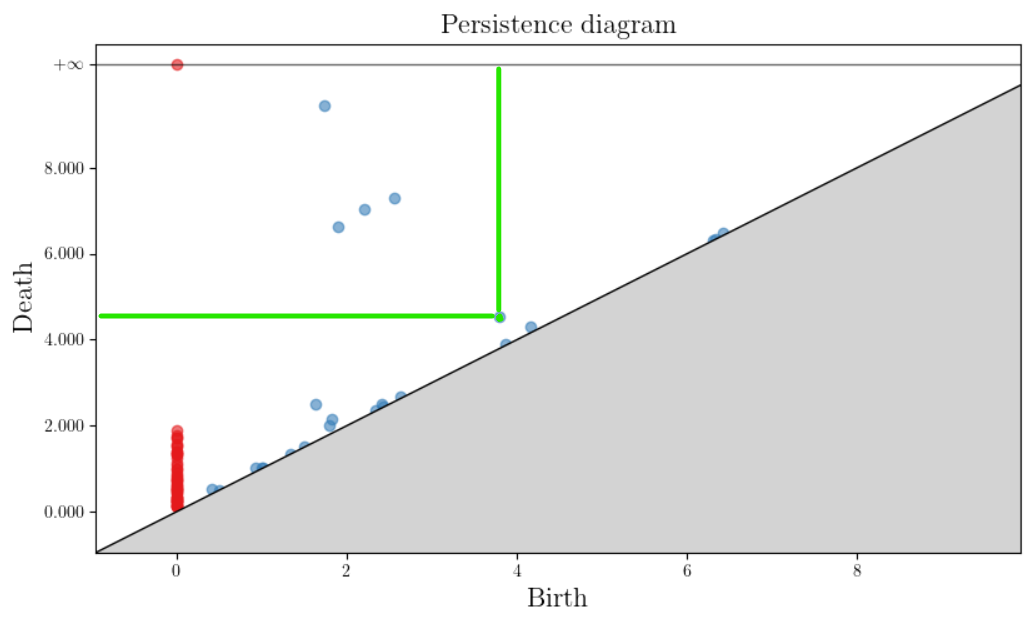
\includegraphics[width=0.7\textwidth]{figures/bg/persistenceEx.png} 
\caption{Persistence diagram, where 0-dimensional persistence homology is in red and 1-dimensional case is in blue. The 1-dimensional persistent Betti number corresponding to the green point is 5.}
\label{ref:persEx}
\end{figure}



\section{Related work}




\section{Summary}

%\engExpl{It is nice to have this chapter conclude with a summary. For example, you can include a table that summarizes other people's ideas and benefits and drawbacks - so that later, you can compare your solution to each of them. This will also help you define the variables that you will use for your evaluation.}

\end{document}